
%(BEGIN_QUESTION)
% Copyright 2007, Tony R. Kuphaldt, released under the Creative Commons Attribution License (v 1.0)
% This means you may do almost anything with this work of mine, so long as you give me proper credit

\noindent
{\bf DANGER!}  {\it The following question will probably shatter your fundamental conceptions about how thermocouples work!  If you find the topic confusing enough already, please turn the page and skip past this question!!}

\vskip 10pt

Everything you thought you knew about thermocouples is wrong.  Well, maybe not {\it everything}, but just the fundamental principle upon which they operate.  In school you probably learned that the Seebeck effect depends on a junction of dissimilar substances, usually two different metals or metal alloys.

\vskip 10pt

Wrong.

\vskip 10pt

In point of fact, the Seebeck effect exists along the length of any {\it one} substance that is differentially heated.  Take this length of copper wire for example, with one end held at the freezing point of water and the other end held at the boiling point of water:

$$\includegraphics[width=15.5cm]{i02977x01.eps}$$

The Seebeck coefficient ($\sigma$) is equal to the derivative of voltage ($V$) with respect to temperature ($T$):

$$\sigma = \lim_{\Delta T \to 0} {\Delta V \over \Delta T}$$

$$\sigma = {dV \over dT}$$

Different substances have different Seebeck coefficients.  The following table shows several common examples:

% No blank lines allowed between lines of an \halign structure!
% I use comments (%) instead, so that TeX doesn't choke.

$$\vbox{\offinterlineskip
\halign{\strut
\vrule \quad\hfil # \ \hfil & 
\vrule \quad\hfil # \ \hfil & 
\vrule \quad\hfil # \ \hfil \vrule \cr
\noalign{\hrule}
%
% First row
Substance & $\sigma$ @ 0$^{o}$ C & $\sigma$ @ 100$^{o}$ C\cr
%
\noalign{\hrule}
%
% Another row
Copper & 1.72 $\mu$V / $^{o}$C & 2.23 $\mu$V / $^{o}$C \cr
%
\noalign{\hrule}
%
% Another row
Silver & 1.42 $\mu$V / $^{o}$C & 1.84 $\mu$V / $^{o}$C \cr
%
\noalign{\hrule}
%
% Another row
Gold & 2.3 $\mu$V / $^{o}$C & 2.0 $\mu$V / $^{o}$C \cr
%
\noalign{\hrule}
%
% Another row
Tungsten & 1.9 $\mu$V / $^{o}$C & 6.7 $\mu$V / $^{o}$C \cr
%
\noalign{\hrule}
%
% Another row
Nickel & -7.0 $\mu$V / $^{o}$C & -12.4 $\mu$V / $^{o}$C \cr
%
\noalign{\hrule}
%
% Another row
Kovar & 0.20 $\mu$V / $^{o}$C & 0.19 $\mu$V / $^{o}$C \cr
%
\noalign{\hrule}
%
% Another row
Silicon & -408 $\mu$V / $^{o}$C & -455 $\mu$V / $^{o}$C \cr
%
\noalign{\hrule}
} % End of \halign 
}$$ % End of \vbox

However, it is impossible to measure this voltage by connecting a real voltmeter across the ends of this copper wire.  Explain why.  Furthermore, explain how a {\it junction} of dissimilar materials may produce a thermal voltage that is easily measured.

\underbar{file i02977}
%(END_QUESTION)





%(BEGIN_ANSWER)

In connecting a room-temperature voltmeter to the ends of the copper wire, we form two more temperature gradients: one from freezing to room temperature, and the other from boiling to room temperature.  Those gradients produce Seebeck voltages directly opposed to the Seebeck voltage across the length of the copper wire, resulting in a complete cancellation and zero voltage registered by the voltmeter.

$$\includegraphics[width=15.5cm]{i02977x03.eps}$$

In other words, from one voltmeter lead to the other, we see a net temperature gradient of zero (from room temperature to room temperature) along the same material (copper), resulting in a net Seebeck voltage of zero.

\vskip 10pt

A {\it junction} of two different metals, on the other hand, produces two unequal Seebeck voltages given the same temperature gradient from end to end along each wire:

$$\includegraphics[width=15.5cm]{i02977x02.eps}$$

We can measure the net Seebeck voltage between the two cold wire ends because they are both at the same temperature as our meter leads.  No temperature gradient exists at the connection point between the thermocouple leads and the meter leads, so no Seebeck voltage is generated here to add to the circuit's net voltage.

%(END_ANSWER)





%(BEGIN_NOTES)

Thermocouple theory is so badly represented in most introductory textbooks that the real Seebeck effect seems alien.  For example, in the answer's illustration with copper and silver wire, we realize there is actually no such thing as a ``reference junction voltage'' as we are commonly taught in thermocouple circuits.  The diminishing of total (net) voltage resulting from a warming reference junction is actually due to less Seebeck voltage generated along the lengths of {\it both} wires from end to end, rather than an increasing reference junction voltage subtracting from a constant measurement junction voltage.

However, the false model of voltages being produced {\it at each junction} instead of along the wires' lengths is so commonly held that it almost does more harm than good to teach technicians what's really going on in lieu of the popular model.  If students were exclusively taught the {\it real} theory of thermocouples and never the popular (inaccurate) theory, most of the industry terminology would be foreign (e.g. ``What does it mean to compensate for the reference junction voltage?''), and these students' ability to function with other instrumentation professionals would be diminished.  However, if an instructor gives equal time to the real theory and the popular theory, you risk hopelessly confusing a lot of students.  It's like teaching students that the Earth orbits the Sun, and also that the Sun orbits the Earth, and that most people are wrong but they have to work in a world where people do business in the language of a wrong theory anyway.

My personal solution is to teach the popular theory, then introduce the real theory with the prefaced warning that weaker students should plug their ears.  Sad, but true.

\vskip 10pt

Data taken from table on page 153 of {\it The Industrial Electronics Handbook}, edited by J. David Irwin, copyright 1996.

%INDEX% Measurement, temperature: thermocouple
%INDEX% Physics, heat and temperature: Seebeck effect

%(END_NOTES)


